\documentclass[11pt,a4paper]{article}
\usepackage[T1]{fontenc}
\usepackage[utf8]{inputenc}
\usepackage{lmodern,microtype}
\usepackage[margin=28mm,headheight=14pt]{geometry}
\usepackage{amsmath,amssymb,amsthm,mathtools}
\usepackage{booktabs,longtable,array,enumitem}
\usepackage{xcolor,tikz}
\usetikzlibrary{arrows.meta,positioning}
\usepackage{listings,fancyhdr,needspace}
\usepackage{xurl}
\usepackage[colorlinks=true,linkcolor=blue!45!black,urlcolor=blue!55!black,citecolor=blue!45!black]{hyperref}
\usepackage{bookmark}
\definecolor{ink}{RGB}{29,48,66}
\definecolor{accent}{RGB}{0,105,120}
\definecolor{light}{RGB}{240,246,248}
\hypersetup{pdftitle={Constructive dimension invariance in iPRA},pdfauthor={Research report prepared for Vladimir Reshetnikov}}
\pagestyle{fancy}\fancyhf{}
\fancyhead[L]{\small Constructive dimension invariance}
\fancyhead[R]{\small iPRA}\fancyfoot[C]{\thepage}
\setlength{\parskip}{4pt}\setlength{\parindent}{1.1em}
\setlength{\emergencystretch}{2em}
\setlist{itemsep=3pt,topsep=5pt}
\lstset{basicstyle=\small\ttfamily,breaklines=true,columns=fullflexible,
frame=single,rulecolor=\color{black!15},backgroundcolor=\color{light},showstringspaces=false}
\newtheorem{theorem}{Theorem}[section]
\newtheorem{lemma}[theorem]{Lemma}
\newtheorem{corollary}[theorem]{Corollary}
\newtheorem{proposition}[theorem]{Proposition}
\theoremstyle{definition}
\newtheorem{definition}[theorem]{Definition}
\newtheorem{remark}[theorem]{Remark}
\newcommand{\N}{\mathbb N}\newcommand{\Z}{\mathbb Z}
\newcommand{\Q}{\mathbb Q}\newcommand{\R}{\mathbb R}
\newcommand{\ipra}{\mathsf{iPRA}}
\newcommand{\dist}{\operatorname{dist}_{\infty}}
\newcommand{\Cell}{\operatorname{cell}}
\newcommand{\Valid}{\operatorname{Valid}}
\newcommand{\Sep}{\operatorname{Sep}}\newcommand{\Small}{\operatorname{Small}}
\newcommand{\CheckCert}{\operatorname{Check}}\newcommand{\Witness}{\operatorname{Witness}}
\newcommand{\one}[1]{\mathbf 1_{#1}}
\newcommand{\norm}[1]{\left\lVert #1\right\rVert_{\infty}}
\newcommand{\floor}[1]{\left\lfloor #1\right\rfloor}
\newcommand{\repo}{\texttt{ProveIt}}
\newcommand{\sha}{\texttt{daade0300022828cdba33a324d987997fee9fa08}}
\begin{document}
\hypersetup{pageanchor=false}
\begin{titlepage}
\vspace*{13mm}
{\color{accent}\large CONSTRUCTIVE TOPOLOGY / FINITE ARITHMETIC\par}
\vspace{12mm}
{\color{ink}\Huge\bfseries Dimension invariance\par}
\vspace{5mm}
{\color{ink}\LARGE\bfseries in intuitionistic primitive\\
recursive arithmetic\par}
\vspace{8mm}
{\Large A finite proof using staggered rational grids\par}
\vspace{15mm}
{\large Prepared for Vladimir Reshetnikov\par}
{\large 15 November 2026\par}
\vfill
\begin{abstract}
We give an explicit, finite obstruction to lowering dimension. For $d\geq1$, let
$F:\{0,\ldots,N\}^{d}\to\Q^{m}$ be a rational table, with $N\geq1$ and
$h>0$. If every pair of opposite source faces has image separation at
least $h$, and every standard Kuhn simplex has image diameter less than
$h/d$, then $d\leq m$. The proof consists of a cubical Sperner parity
calculation and rational floor computations on $d$ differently shifted
grids. It yields a primitive recursive procedure which, when $d>m$,
returns either a close opposite-face pair or a simplex with large image
variation.

From this finite theorem we derive approximate opposite-face collisions
for uniformly presented maps, and dimension invariance for homeomorphisms
given with primitive recursive rational evaluations and local uniform
continuity moduli for both directions. We state the precise first-order
arithmetic schema, identify the quantifier-free induction invariants,
and explain how to construct an object-language derivation using the
existing \texttt{ConciseIPRA} development.

The human-readable mathematical argument is complete. The accompanying
Lean file is a detailed, explicitly unfinished formalization blueprint.
The exact-arithmetic Python artifacts are executable checks and witness
extractors; they are not a substitute for a Lean or iPRA proof certificate.
\end{abstract}
\vspace{7mm}
{\small Repository audit pinned to \sha.\par}
\end{titlepage}
\hypersetup{pageanchor=true}
\setcounter{tocdepth}{1}
\tableofcontents
\newpage

\section{The statement, its constructive meaning, and its scope}
\subsection{The classical target}
The dimension invariance theorem in the question states
\[
             \R^n\cong\R^m \quad\Longleftrightarrow\quad n=m,
\]
where $\cong$ means homeomorphism \cite{mathworld}. The implication from
right to left is the identity map. The content is that two mutually
inverse continuous maps cannot change the number of coordinates.

An assertion quantifying over arbitrary real spaces and arbitrary
functions between them is not literally a formula of first-order
arithmetic. In this report the internal result is a theorem about
natural-number codes of finite rational tables. Its interpretation for
maps is a schema for \emph{fixed primitive recursive evaluation and
modulus procedures}. This distinction is part of the statement.

We prove three results, in order.
\begin{enumerate}
\item \textbf{Finite obstruction.} A rational table with well-separated
opposite faces and sufficiently small variation on each small simplex
cannot have fewer target coordinates than source coordinates.
\item \textbf{Approximate collision.} Given a uniformly presented map
from a $d$-cube to an $m$-dimensional space with $d>m$, and a requested
positive dyadic tolerance, a primitive recursive construction produces
rational points on opposite faces whose images are closer than that
tolerance.
\item \textbf{Constructive dimension invariance.} A homeomorphism
presented with the evaluation and uniformity data specified below has
equal source and target dimensions. Only one fixed accuracy of the
inverse modulus is needed for each direction.
\end{enumerate}
The second assertion does not construct an exact coincidence point and
does not claim that witnesses at successive accuracies converge. The
third assertion needs neither of those stronger conclusions.

\subsection{Why the supplied moduli matter}
A pointwise assertion of continuity is not used to manufacture a
uniform modulus. The relevant uniformity data are hypotheses. This is
a substantive constructive distinction: Kihara proved that the
unrestricted assertions forbidding continuous injections, or topological
embeddings, from higher-dimensional Euclidean spaces into
lower-dimensional ones are equivalent to weak K\"onig's lemma over
$\mathsf{RCA}_0$ \cite[Theorem 1]{kihara}. His paper separately poses the
homeomorphism-only question; its embedding result must not be
misreported as that stronger classification.

Our result concerns explicitly uniform presentations and does not
assert a new solution to those reverse-mathematical questions. The
finite theorem itself has no continuity or compactness assumption.
It is an ordinary universally quantified arithmetic statement with
primitive recursive predicates.

\subsection{Relationship to existing arguments}
The cubical boundary convention used here is the one in the
Kulpa--M\"uger treatment of Sperner's lemma
\cite[Section 2]{muger}. The separation argument motivates assigning
different boundary grids to different source directions. Here this
idea is implemented entirely with finite sets of rational cells and
explicit spacing. There is no passage from small simplices to a limit
point. The arithmetic construction and all constants are proved below;
no claim of historical priority is made.

The \repo\ material is used for its formal arithmetic and interpretation
interfaces. We do not import an unverified topological theorem from
an archived draft. Section~\ref{sec:repo} records what was inspected.

\section{Finite data and the main quantitative theorem}
\subsection{Grids, norms, and rational tables}
For $d\in\N$ and $N\geq1$, put
$G_d(N)=\{0,\ldots,N\}^{d}$.
We use integer coordinates for the finite argument. When the grid is
used to sample the unit cube, the point represented by $v$ is $v/N$.
For $i=1,\ldots,d$, the lower and upper $i$-faces are
\[
 L_i=\{v\in G_d(N):v_i=0\},\qquad
 U_i=\{v\in G_d(N):v_i=N\}.
\]
For rational vectors $y,z\in\Q^m$, define
$\dist(y,z)=\max_{1\leq j\leq m}|y_j-z_j|$.
The value is defined to be $0$ for $m=0$. Every comparison in the
finite proof is a comparison of rationals, hence decidable by integer
cross-multiplication with positive denominators.

A \emph{Kuhn $d$-simplex} is specified by
$a\in\{0,\ldots,N-1\}^{d}$ and a permutation
$\pi=(\pi_1,\ldots,\pi_d)$ of $\{1,\ldots,d\}$. Its ordered vertices are
\begin{equation}\label{eq:kuhn}
 v_t=a+\sum_{s=1}^{t}e_{\pi_s},\qquad 0\leq t\leq d.
\end{equation}
All its vertices differ by at most one in each coordinate. There are
$N^d d!$ such simplices. When $d=0$, there is one empty tuple and one
zero-dimensional simplex. No geometric realization of a triangulation
is needed: the vertex lists and their facet incidences suffice.

\begin{definition}
Let $F:G_d(N)\to\Q^m$ be a table and $h\in\Q_{>0}$.
The \emph{opposite-face separation condition} is
\begin{equation}\label{eq:sep}
 \dist(F(u),F(v))\geq h
 \quad(i=1,\ldots,d,\ u\in L_i,\ v\in U_i).
\end{equation}
For $d>0$, the \emph{small-simplex condition} is
\begin{equation}\label{eq:small}
 \dist(F(u),F(v))<h/d
 \quad(u,v\hbox{ vertices of the same Kuhn simplex}).
\end{equation}
Equivalently, the latter condition is $d\,\dist(F(u),F(v))<h$.
\end{definition}

\begin{theorem}[Finite dimension obstruction]\label{thm:finite}
If $d>0$, $N\geq1$, $h>0$, and the rational table $F$ satisfies
\eqref{eq:sep} and \eqref{eq:small}, then $d\leq m$.
For $d=0$, the conclusion is automatic.
\end{theorem}
The theorem has a positive version, with an explicit witness.
\Needspace{10\baselineskip}
\begin{theorem}[Finite witness alternative]\label{thm:alternative}
For every valid rational table $F:G_d(N)\to\Q^m$ with $d>m$,
$N\geq1$ and $h>0$, a primitive recursive procedure returns one of:
\begin{enumerate}[label=\textup{(\roman*)}]
\item an index $i$ and points $u\in L_i$, $v\in U_i$ such that
      $\dist(F(u),F(v))<h$;
\item a Kuhn simplex and two of its vertices $u,v$ such that
      $\dist(F(u),F(v))\geq h/d$.
\end{enumerate}
The returned data can be checked using rational arithmetic alone.
\end{theorem}
We prove the finite alternative directly. The obstruction follows
by excluding both alternatives. The strict inequality in
\eqref{eq:small} is intentional; applications preserve it with slack.

\section{A complete finite cubical Sperner argument}\label{sec:sperner}
\subsection{Boundary conditions}
Let $\lambda:G_d(N)\to\{0,\ldots,d\}$. Call it \emph{admissible} if
\begin{align}
 v_i=0 &\quad\Longrightarrow\quad \lambda(v)<i,\label{eq:lower}\\
 v_i=N &\quad\Longrightarrow\quad \lambda(v)\ne i-1.\label{eq:upper}
\end{align}
Coordinates are numbered $1,\ldots,d$ and colors $0,\ldots,d$.
In the executable code coordinates are numbered from zero; the
corresponding conditions are $\lambda(v)\leq i$ on the lower face
and $\lambda(v)\ne i$ on the upper face.
A $d$-simplex is \emph{full} if its vertices have exactly the
colors $0,\ldots,d$, each once.

\begin{theorem}[Cubical parity lemma]\label{thm:sperner}
For every admissible labeling, the number of full Kuhn $d$-simplices
is odd. A full simplex is therefore found by a bounded search
through $N^d d!$ entries.
\end{theorem}

\subsection{Facet incidences without a geometric theorem}
Assume $d\geq1$. The facet occurrence $(a,\pi,t)$ is the vertex list of
\eqref{eq:kuhn} with $v_t$ removed. The following explicit rules pair
every interior occurrence with its unique other occurrence.
\begin{enumerate}
\item If $0<t<d$, keep $a$, exchange $\pi_t$ and $\pi_{t+1}$,
and again remove vertex $t$. Only the removed intermediate vertex
changes; the other vertices are identical.
\item If $t=0$, take base $a+e_{\pi_1}$, permutation
$(\pi_2,\ldots,\pi_d,\pi_1)$, and remove its last vertex.
This is valid precisely when $a_{\pi_1}<N-1$.
If $a_{\pi_1}=N-1$, the original facet lies on the upper
$\pi_1$-face and has no mate inside the grid.
\item If $t=d$, take base $a-e_{\pi_d}$, permutation
$(\pi_d,\pi_1,\ldots,\pi_{d-1})$, and remove its first vertex.
This is valid precisely when $a_{\pi_d}>0$.
If $a_{\pi_d}=0$, the original facet lies on the lower
$\pi_d$-face and has no mate inside the grid.
\end{enumerate}
These rules are mutually inverse and never pair an occurrence with
itself. They exhaust the possibilities. Order the vertices of a
facet by the sum of their coordinates. Along a simplex this sum
increases by one at every step. If an interior vertex was removed,
there is one gap of two, and the missing two unit increments can
occur in exactly two orders. If an endpoint was removed, the
remaining increments use $d-1$ different coordinates. The missing
coordinate can be added only at the start or at the end.
This also proves uniqueness of the mate.

Every coordinate varies on an interior-deletion facet. On an
endpoint-deletion facet the omitted increment determines its
only constant coordinate. Thus the unpaired occurrences are exactly
the boundary facets. For $d=1$ the same rules pair the endpoints of
adjacent intervals, leaving $0$ and $N$ unpaired.

\subsection{Counting doors}
For $d\geq1$, call a facet a \emph{door} if its $d$ vertices have
exactly the colors $0,\ldots,d-1$. A fixed $d$-simplex has:
\begin{itemize}
\item one door if it is full: remove its color-$d$ vertex;
\item no door if some color among $0,\ldots,d-1$ is absent;
\item two doors otherwise: color $d$ is absent, exactly one
remaining color is repeated, and either copy can be removed.
\end{itemize}
Thus the parity of the number of door occurrences equals the
parity of the number of full $d$-simplices.

Interior doors occur in pairs and contribute an even number.
A boundary door cannot lie on an upper $i$-face, because color
$i-1$ is forbidden there. It cannot lie on a lower $i$-face with
$i<d$, because all colors there are less than $i$, so color $d-1$
is absent. Only the lower $d$-face can contain boundary doors.

Delete the final coordinate on that face. Its facets are exactly
the Kuhn $(d-1)$-simplices of $G_{d-1}(N)$. Conversely, each such
simplex is the last-deletion facet of the $d$-simplex obtained by
appending coordinate $d$ to its permutation and setting the last
base coordinate to zero. The restricted labeling takes values in
$\{0,\ldots,d-1\}$ and satisfies the boundary conditions in the
remaining coordinates. Therefore
\begin{equation}\label{eq:parity}
 \#\{\hbox{full $d$-simplices}\}
 \equiv
 \#\{\hbox{full $(d-1)$-simplices on the lower $d$-face}\}
 \pmod2.
\end{equation}
In dimension zero the single vertex has color zero and is full.
Iterating \eqref{eq:parity} proves that the top-dimensional count
is odd, proving Theorem~\ref{thm:sperner}.

\subsection{The induction is genuinely quantifier-free}
In $\ipra$ we do not induct on the formula asserting that
\emph{every labeling of every $r$-cube} has odd parity; that formula
has unbounded quantifiers.

Fix the original data $d,N,\lambda$ as numerical parameters.
For $0\leq r\leq d$, restrict $\lambda$ to
$x_{r+1}=\cdots=x_d=0$. For $r<d$, \eqref{eq:lower} with
$i=r+1$ forces all restricted colors to be at most $r$.
Let $P(r)$ be the parity of the full $r$-simplex count on this
fixed restricted table, with the default value zero for $r>d$.
It is a primitive recursive function of
$r,d,N,\lambda$. The double count gives $P(r+1)=P(r)$ for $r<d$,
and $P(0)=1$. Quantifier-free induction on
\[
                 r\leq d\ \longrightarrow\ P(r)=1
\]
suffices. The relation $r\leq d$ is also a characteristic-function
equation. For $r\geq d$ the next guarded statement is vacuous.
The coloring assumptions remain fixed hypotheses, outside the
induction formula.

All subsidiary counts use bounded lists. An involution without
fixed points has even cardinality because each pair has a unique
smaller index: its cardinality is twice the number of those indices.
This equality is a bounded indicator-sum calculation. Thus parity
cancellation does not invoke unrestricted induction.

\section{Staggered rational cells and the dimension obstruction}
\subsection{One grid for each source direction}
Assume $d>0$, $h>0$, and put $s_i=(i-1)/d$ for $i=1,\ldots,d$.
For rational $y\in\Q^m$ define
\begin{equation}\label{eq:cell}
 \Cell_i(y)=
 \left(\floor{\frac{y_j}{h}-s_i}\right)_{j=1}^{m}\in\Z^m.
\end{equation}
The one-dimensional cells are the half-open intervals
\[
        [\,h(k+s_i),\,h(k+1+s_i)\,),\qquad k\in\Z.
\]
The half-open convention makes membership unambiguous even at
an exact boundary. Floors are taken only of rational samples.

\begin{lemma}[Elementary cell facts]\label{lem:cells}
\leavevmode
\begin{enumerate}[label=\textup{(\roman*)}]
\item Equal cell tuples imply $\dist(y,z)<h$.
\item If the $j$th cell indices differ, a computable threshold
$t=h(k+s_i)$ satisfies
$\min(y_j,z_j)<t\leq\max(y_j,z_j)$.
\item Boundaries belonging to distinct grids $i\ne i'$ in one
target coordinate are separated by at least $h/d$.
\end{enumerate}
\end{lemma}
\begin{proof}
Two points in the same half-open interval of length $h$ differ
by less than $h$. Their finite coordinate maximum is less than
$h$ as well. For $m=0$, the distance is zero.

For (ii), take $k$ to be one plus the smaller cell index.
The sample in that cell is strictly below $h(k+s_i)$, and
the sample in the higher cell is at least that number.

For (iii), subtract two boundaries:
\begin{equation}\label{eq:latticegap}
 h(k+s_i)-h(k'+s_{i'})
       =\frac hd\bigl(d(k-k')+i-i'\bigr).
\end{equation}
The integer in parentheses is nonzero: otherwise $d$ would
divide $i-i'$, whereas $0<|i-i'|<d$. Its absolute value is
at least one, giving the asserted spacing.
\end{proof}

\subsection{Coloring from the lower faces}
Suppose opposite-face separation \eqref{eq:sep} holds. Form
\[
        S_i=\{\Cell_i(F(w)):w\in L_i\}.
\]
No bound on the target image is needed: this is a finite list
of integer tuples. Define
\[
 b_i(v)=
 \begin{cases}
 0,&\Cell_i(F(v))\in S_i,\\
 1,&\Cell_i(F(v))\notin S_i.
 \end{cases}
\]
Membership is decided by a finite scan. On the lower $i$-face
the bit is zero, using $w=v$. On the upper $i$-face it is one:
otherwise a lower-face point would be in the same cell,
contradicting separation by Lemma~\ref{lem:cells}(i).

Give $v$ the color
\begin{equation}\label{eq:color}
 \lambda(v)=
 \begin{cases}
 i-1,&i\text{ is the least index with }b_i(v)=0,\\
 d,&b_1(v)=\cdots=b_d(v)=1.
 \end{cases}
\end{equation}
On a lower $i$-face the first zero occurs no later than $i$,
so the color is less than $i$. On an upper $i$-face bit $i$
is one, so the color cannot be $i-1$. This is an admissible
labeling.

\subsection{A full simplex forces separated thresholds}
Choose a full Kuhn simplex $\sigma$ by
Theorem~\ref{thm:sperner}. Let $v^{(r)}$ be its vertex of color
$r$. At $v^{(d)}$ all bits are one. At $v^{(i-1)}$ bit $i$
is zero. Consequently
\[
       \Cell_i(F(v^{(i-1)}))
       \ne \Cell_i(F(v^{(d)})).
\]
Select the least differing coordinate $j_i$. When $m=0$ the
two empty tuples cannot differ; indeed separation already
fails then. We may assume $m>0$.

Compute a threshold $t_i$ from grid $i$ between the two
indicated coordinates, by Lemma~\ref{lem:cells}(ii). Put
\[
 I_j=\left[\min_{v\in\sigma}F(v)_j,\
                  \max_{v\in\sigma}F(v)_j\right].
\]
Every $t_i$ lies in $I_{j_i}$. Under \eqref{eq:small}, each
$I_j$ has length less than $h/d$. Distinct indices cannot
have $j_i=j_{i'}$, since their thresholds would differ by at
least $h/d$. We have an injection of $d$ source directions
into $m$ target coordinates, hence $d\leq m$. This proves
Theorem~\ref{thm:finite}.

The finite pigeonhole step has a direct arithmetic proof:
let $c_j=\sum_{i=1}^d\one{j_i=j}$. Distinctness implies
$c_j\leq1$, while exchanging finite sums gives
$\sum_{j=1}^m c_j=d$. Hence $d\leq m$.

\subsection{Extracting the positive alternative}
For $d>m$, first scan all opposite-face pairs. Return the first
pair at distance less than $h$, if found. Otherwise separation
holds, by decidability of those finitely many rational comparisons.
Construct the coloring, select a full simplex, and compute
its $d$ thresholds.

Find the first repeated coordinate in $j_1,\ldots,j_d$; the
finite sum argument proves that one exists. If
$j_i=j_{i'}=j$, then $|t_i-t_{i'}|\geq h/d$.
Both thresholds lie in $I_j$. Select a vertex attaining
the minimum of $F(v)_j$ on $\sigma$ and one attaining the
maximum. Their coordinate difference, and thus their sup
distance, is at least $h/d$. Return them with the base and
permutation defining $\sigma$.
This bounded construction proves Theorem~\ref{thm:alternative}.

\section{A small worked example}
Take $d=2$, $m=1$, $N=1$, $h=1$, and
\[
 F(0,0)=0,\quad F(0,1)=1,\quad F(1,0)=3,\quad F(1,1)=2.
\]
The first pair of opposite faces has image sets $\{0,1\}$ and
$\{3,2\}$; the second has $\{0,3\}$ and $\{1,2\}$.
Both separations are at least one.

Grid one has integer boundaries; grid two has half-integer
boundaries. The occupied lower-face cell indices are
$S_1=\{0,1\}$ and $S_2=\{-1,2\}$. The colors at
$(0,0),(0,1),(1,0),(1,1)$ are $0,0,1,2$, respectively.
The simplex $(0,0),(1,0),(1,1)$ is full.

\begin{figure}[ht]
\centering
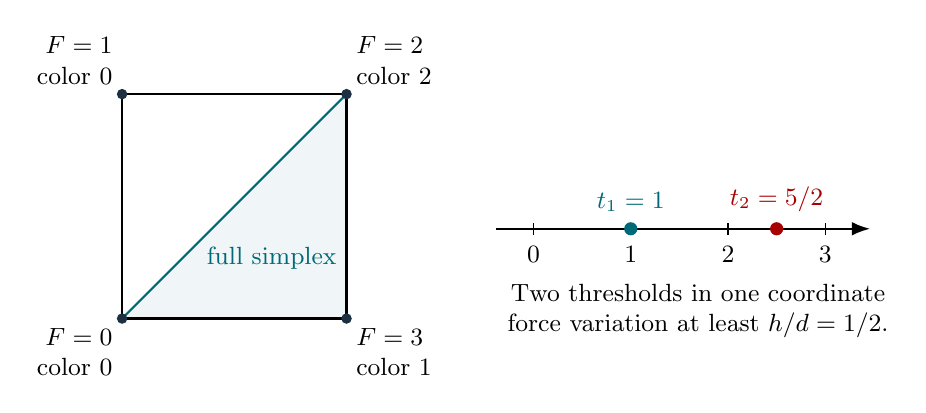
\begin{tikzpicture}[scale=.95,every node/.style={font=\small}]
 \fill[accent!6] (0,0)--(3,0)--(3,3)--cycle;
 \draw[thick] (0,0) rectangle (3,3);
 \draw[thick,accent] (0,0)--(3,3);
 \foreach \x/\y in {0/0,3/0,0/3,3/3}
   \fill[ink] (\x,\y) circle (2pt);
 \node[below left,align=right] at (0,0) {$F=0$\\color $0$};
 \node[below right,align=left] at (3,0) {$F=3$\\color $1$};
 \node[above left,align=right] at (0,3) {$F=1$\\color $0$};
 \node[above right,align=left] at (3,3) {$F=2$\\color $2$};
 \node[accent] at (2,.8) {full simplex};
 \draw[-{Latex},thick] (5,1.2)--(10,1.2);
 \foreach \t/\lab in {5.5/0,6.8/1,8.1/2,9.4/3}{
   \draw (\t,1.12)--(\t,1.28);
   \node[below] at (\t,1.1) {$\lab$};
 }
 \fill[accent] (6.8,1.2) circle (2.5pt);
 \fill[red!65!black] (8.75,1.2) circle (2.5pt);
 \node[above,accent] at (6.8,1.3) {$t_1=1$};
 \node[above,red!65!black] at (8.75,1.3) {$t_2=5/2$};
 \node[align=center] at (7.7,.1) {Two thresholds in one coordinate\\
 force variation at least $h/d=1/2$.};
\end{tikzpicture}
\caption{A two-dimensional finite source and its one-dimensional target.}
\end{figure}

With the common color-$2$ vertex, the first threshold is $1$,
between image values $0$ and $2$. The second is $5/2$, between
image values $3$ and $2$. They use the only target coordinate.
The simplex has image range $[0,3]$, giving variation at least
$1/2$. This is the accompanying JSON example. It illustrates
the second alternative, not a continuous embedding.

\section{Primitive recursive implementation and finite certificates}
\subsection{Explicit search bounds}
Write $V=(N+1)^d$ and $S=N^d d!$. There are $V$ vertices,
$S$ Kuhn simplices, and $(N+1)^{d-1}$ vertices on each face
when $d>0$. The following simple bounds suffice.

\begin{center}
\begin{tabular}{p{.48\textwidth}p{.38\textwidth}}
\toprule
Operation & Candidates or comparisons\\
\midrule
Enumerate vertices & $V$\\
Check opposite-face pairs & $d(N+1)^{2d-2}$ pairs\\
Compute all cell tuples & $dVm$ rational floors\\
Test all occupied-cell memberships & at most $dV^2m$ integer comparisons\\
Find a full simplex & at most $S$ vertex lists\\
Choose differing coordinates & at most $dm$ comparisons\\
Find a repeated coordinate & at most $d^2$ comparisons\\
Choose extrema within a simplex & at most $2(d+1)$ comparisons\\
\bottomrule
\end{tabular}
\end{center}

One may enumerate permutations by testing all $d$-tuples with
entries below $d$ for distinctness. This gives the even simpler
primitive recursive search bound $d^d$ instead of $d!$.
Dimension zero is handled separately. These bounds establish
primitive recursiveness, not practical efficiency.

Integer arithmetic, exponentiation, bounded sums and products,
bounded search, and rational floor are primitive recursive.
The largest numerator and denominator in the input table are
obtained by bounded maxima. All intermediate numbers arise
from boundedly many additions and multiplications and
divisions with explicit positive denominators. Their sizes
therefore have primitive recursive bounds in the input code
and the displayed loop bounds.

\subsection{A concrete coding convention}
Code a signed integer by $z\mapsto2z$ for $z\geq0$ and
$z\mapsto-2z-1$ for $z<0$. A rational is a pair
$(\operatorname{code}(a),b)$ with $b>0$, denoting $a/b$.
Reduction to lowest terms is unnecessary.
A possible pairing function is
\[
        \langle x,y\rangle=\frac{(x+y)(x+y+1)}2+y.
\]
Its projections are computed by bounded search with both
components at most the input code. Code a list by its length
and an iterated pairing of its entries. Access, replacement,
concatenation, and finite folds are primitive recursive.
Malformed inputs receive fixed defaults, and a validity
predicate guards every theorem.

For $a/b$ with $b>0$, signed division gives the integer $q$
such that $qb\leq a<(q+1)b$. Search for it in
$[-(|a|+1),|a|+1]$. Existence and uniqueness are the usual
integer-division calculation, proved by quantifier-free
induction. Thus negative coordinates and exact endpoints
introduce no nonconstructive operation.

\subsection{The independent checker}
A certificate of the first kind is $(i,u,v)$. Check grid
membership, the face equations, and
$\dist(F(u),F(v))<h$.

A certificate of the second kind is $(a,\pi,u,v)$. Check the
base and permutation, reconstruct its vertices, check that
$u,v$ occur, and verify $d\,\dist(F(u),F(v))\geq h$.

The extraction code also prints colors and thresholds for
inspection. The checker does not trust that trace; the final
finite witness is enough. Acceptance establishes that
particular rational witness. It does not establish the
general theorem or the proof's arithmetic strength.

\section{From rational tables to approximate face collisions}
\subsection{What a uniform presentation supplies}
Let $C_d=[0,1]^d$ and interpret $f:C_d\to\R^m$
constructively. It is enough to have:
\begin{enumerate}
\item a fixed primitive recursive procedure $A(q,p)\in\Q^m$
for rational $q\in C_d$, satisfying
\begin{equation}\label{eq:eval}
                 \norm{A(q,p)-f(q)}\leq2^{-p};
\end{equation}
\item a fixed primitive recursive uniform modulus $\mu$ such
that, at least for rational $q,q'\in C_d$,
\begin{equation}\label{eq:modulus}
 \norm{q-q'}\leq2^{-\mu(k)}
       \quad\Longrightarrow\quad
 \norm{f(q)-f(q')}\leq2^{-k}.
\end{equation}
\end{enumerate}
There is no test of real equality. The real notation is
interpretive shorthand; the next section gives a completely
arithmetical version sufficient for the argument.

\begin{theorem}[Effective approximate face collision]\label{thm:collision}
If $d>m$ and $f$ has this presentation, then for every
$a\in\N$ a primitive recursive construction produces
$i$ and rational $q,q'\in C_d$ such that
\[
 q_i=0,\quad q'_i=1,\qquad
                  \norm{f(q)-f(q')}<2^{-a}.
\]
The fixed definitions of $A,\mu$ are composed into the
resulting primitive recursive procedure.
\end{theorem}
\begin{proof}
Set
\begin{equation}\label{eq:scales}
 \delta=2^{-a},\quad k=a+d+3,\quad p=k+1,\quad
 N=2^{\mu(k)},\quad h=\delta/2,
\end{equation}
and sample $F(v)=A(v/N,p)$ on $G_d(N)$.
Vertices of one Kuhn simplex have source distance at most
$1/N=2^{-\mu(k)}$. The modulus and the two evaluation
errors give sample distance at most
\begin{equation}\label{eq:smallbound}
 2^{-k}+2\cdot2^{-p}
 =2^{1-k}
 =\frac{\delta}{2^{d+2}}
 \leq\frac{\delta}{4d}
 <\frac{\delta}{2d}
 =\frac hd.
\end{equation}
We used $d\geq1$ and $d\leq2^d$.

Theorem~\ref{thm:alternative} cannot return a large-variation
simplex. It therefore returns opposite-face vertices $u,v$
whose sample distance is less than $h$. Put $q=u/N$,
$q'=v/N$. Since $k\geq a+4$,
\begin{align*}
 \norm{f(q)-f(q')}
 &\leq\dist(F(u),F(v))+2^{1-p}\\
 &<\frac{\delta}{2}+2^{-k}
 \leq\frac{\delta}{2}+\frac{\delta}{16}
 =\frac{9\delta}{16}<\delta.
\end{align*}
The strict inequality has explicit rational slack; no
decision of real order was made.
\end{proof}

The procedure does not search for a modulus or for an unknown
convergence stage. Grid size and evaluation precision are
fixed before sampling by \eqref{eq:scales}.

\section{The exact first-order arithmetic schema}\label{sec:schema}
\subsection{Two numerical hypotheses}
Fix primitive recursive symbols $A,\mu$. Tuples, dimensions
and any additional parameters are natural-number codes.
Require valid rational $m$-tuple outputs for valid rational
$q\in C_d$. In readable notation the forward hypothesis is
\begin{equation}\label{eq:U}
\begin{split}
 &\text{for all rational }q,q'\in C_d\text{ and all }k,p,\\
 &\norm{q-q'}\leq2^{-\mu(k)}
 \ \Longrightarrow\
 \dist(A(q,p),A(q',p))\leq2^{-k}+2^{1-p}.
\end{split}
\end{equation}
The one-scale inverse hypothesis, with numerical parameter
$a\in\N$, is
\begin{equation}\label{eq:I}
\begin{split}
 &\text{for all rational }q,q'\in C_d\text{ and all }p,\\
 &\dist(A(q,p),A(q',p))+2^{1-p}<2^{-a}
 \ \Longrightarrow\
 \norm{q-q'}\leq\tfrac12.
\end{split}
\end{equation}
All tuple restrictions are primitive recursive tests.
These are first-order formulas for each fixed choice of
procedures. Their leading universal quantifiers are numerical
quantifiers, and the formulas are hypotheses of a theorem,
not induction formulas.

\begin{theorem}[Arithmetic dimension schema]\label{thm:schema}
For each fixed primitive recursive $A,\mu$, $\ipra$ proves
that output validity and \eqref{eq:U}, \eqref{eq:I} imply
$d\leq m$.
\end{theorem}
\begin{proof}
Dimension zero is immediate. By decidable natural-number
comparison, consider $d>m$, and take \eqref{eq:scales}.
Hypothesis \eqref{eq:U} proves \eqref{eq:smallbound} for
$F(v)=A(v/N,p)$. The finite alternative supplies opposite
$u,v$ with sample distance less than $h$. The rational
calculation
\[
 \dist(A(u/N,p),A(v/N,p))+2^{1-p}
           <\tfrac{9}{16}2^{-a}<2^{-a}
\]
activates \eqref{eq:I}. It gives $\norm{u/N-v/N}\leq1/2$.
But their $i$th coordinates are zero and one, so that
distance is exactly one. The contradiction excludes the
decidable alternative $d>m$, yielding $d\leq m$.
\end{proof}
This proof contains no real numbers. It never infers a
positive real gap merely from a negated real inequality.

\subsection{A schema, not a universal evaluator}
The symbols $A,\mu$ stand for fixed primitive recursive
definitions, possibly with numerical parameters. The
theorem is uniform in those parameters. Concrete definitions
may be substituted when their hypotheses are established.

We do not claim a single primitive recursive evaluator for
all primitive recursive program codes on all inputs. Such
an unrestricted evaluator would be contradicted by the
usual diagonal function obtained by adding one to its value
on the diagonal. A bounded step-limited evaluator with a
supplied clock is a different construction, and is not
needed here.

Nor do we quantify internally over arbitrary infinite
streams. The finite theorem is one arithmetic theorem;
the map interpretation is a schema for fixed procedures.
An oracle-relative version of the finite argument can be
stated separately, but is not an unrelativized first-order
$\ipra$ theorem.

\section{Constructive invariance of Euclidean dimension}
\subsection{The inverse information actually needed}
Suppose $f:C_d\to\R^m$ has \eqref{eq:eval}--\eqref{eq:modulus}
and a supplied integer $a$ satisfies
\begin{equation}\label{eq:inverse-real}
 \norm{f(q)-f(q')}<2^{-a}
       \ \Longrightarrow\
 \norm{q-q'}\leq\tfrac12
 \qquad(q,q'\in C_d\cap\Q^d).
\end{equation}
This follows from a uniformly continuous left inverse on
the image: use its modulus at output tolerance $1/2$,
and $g(f(q))=q$. The integer is supplied, not extracted
from arbitrary pointwise continuity.

Evaluation error and \eqref{eq:inverse-real} give \eqref{eq:I}.
Forward uniformity gives \eqref{eq:U}. Theorem~\ref{thm:schema}
therefore gives $d\leq m$. Equivalently,
Theorem~\ref{thm:collision} contradicts \eqref{eq:inverse-real}
when $d>m$.

\begin{definition}[Locally uniformly presented homeomorphism]
For this theorem a homeomorphism $f:\R^n\to\R^m$ with inverse
$g$ is supplied with fixed primitive recursive rational
approximation procedures and uniform continuity moduli on
specified bounded boxes. The inverse identities and uniform
inverse information on the images of the chosen cubes are
part of the presentation.

Only one positive-size rational cube in each source space
is needed. The internal proof uses the rational-sample
consequences \eqref{eq:U} and \eqref{eq:I}; those consequences
may instead be supplied directly.
\end{definition}

Here boxwise moduli for the interpreted inverse apply to its
actual input points, including possibly irrational images $f(q)$.
A modulus stated only for rational inputs must first be extended
to the represented real map, or \eqref{eq:I} supplied directly.
The inverse information can then be obtained from boxwise moduli
for $g$ and a numerical box containing $f(C_n)$, and
symmetrically for $f$. A containing box can be produced
by a finite mesh estimate. Take a grid of spacing
$2^{-\mu(0)}$, evaluate at precision $1$, let $M$ be the
largest sample sup norm, and use the integer radius
$B=\lceil M+3/2\rceil+1$. Every rational source point is
within one mesh spacing of a vertex, and its image is
within $1+1/2$ of the sample by the modulus and evaluation
error. Thus the required rational images lie in that box.
If uniformity is also specified on all constructive real
inputs, the same estimate extends to them by approximation.
Only the rational version is used in the proof.

\begin{corollary}[Constructive dimension invariance]\label{cor:dimension}
For locally uniformly presented Euclidean spaces and
homeomorphisms in this sense,
\[
                  \R^n\cong\R^m\quad\Longleftrightarrow\quad n=m.
\]
Each instance of the nontrivial implication follows from
the arithmetic schema of Theorem~\ref{thm:schema}.
\end{corollary}
\begin{proof}
Apply the schema to $f$ on a chosen $n$-cube, after
explicit rational affine rescaling if needed, to get
$n\leq m$. Apply it to $g$ on an $m$-cube to get
$m\leq n$. Antisymmetry gives $n=m$.
If one dimension is zero, the positive-dimensional
direction already excludes a map with the stated inverse
data into a singleton.
When $n=m$, the identity has exact rational evaluations,
modulus $\mu(k)=k$, and an immediate inverse modulus;
it gives the constructive converse.
\end{proof}

\subsection{Scope of the conclusion}
The proof does not require differentiability, Lipschitz
bounds, a piecewise linear input map, or an extension of
the inverse to an ambient neighborhood.

It does not produce an exact common image point, prove a
general fixed point theorem or invariance of domain, or
derive uniform continuity from arbitrary pointwise
continuity. None of these assertions is needed.

Classically, a homeomorphism and its inverse have the needed
uniformity on the relevant compact images. The same finite
argument with those classical witnesses gives the usual
dimension theorem. This observation does not make arbitrary
classical functions primitive recursively evaluable, and
does not attribute classical compactness to $\ipra$.

\section{Why the finite proof fits in iPRA}\label{sec:ipra}
\subsection{The theory}
We use first-order intuitionistic logic with equality, symbols
for fixed primitive recursive functions, their defining
equations, successor injectivity and successor/zero separation,
and induction restricted to quantifier-free formulas.
This is the theory implemented by
\texttt{ConciseIPRA.PR} \cite{proveit-pr}.

Numerical predicates used for case distinctions have Boolean
characteristic functions. A finite universal assertion is a
conjunction fold, and a finite existential assertion is a
disjunction fold. Their correctness is proved using
quantifier-free induction on a scan index.
Thus bounded quantifiers in the exposition abbreviate
primitive recursive operations; they do not enlarge the
induction schema.

\subsection{The internal theorem}
Let $\Valid(d,m,N,h,T)$ check table dimensions, positive
denominators, $N\geq1$, and $h>0$. Let $\Sep$ and $\Small$
be the Boolean scans of \eqref{eq:sep} and $d\,\dist<h$
over the explicit finite lists. Define smallness to be true
for $d=0$. The finite obstruction has the form
\begin{equation}\label{eq:internal}
 \forall d,m,N,h,T\quad
  (\Valid=1\wedge\Sep=1\wedge\Small=1
                         \ \longrightarrow\ d\leq m).
\end{equation}
All symbols in the matrix are fixed primitive recursive
symbols or Boolean combinations of equations.

Let $\Witness$ implement the procedure in Section~4.4,
with default output on malformed inputs, and let $\CheckCert$
be the two-tag certificate verifier. The stronger theorem is
\begin{equation}\label{eq:internal-witness}
\begin{split}
 \forall d,m,N,h,T\quad
 (&\Valid(d,m,N,h,T)=1\wedge d>m\\
  &\Longrightarrow
  \CheckCert(d,m,N,h,T,\Witness(d,m,N,h,T))=1).
\end{split}
\end{equation}
The two output tags realize a disjunction with its witness.
No double-negation elimination for an unbounded existential
is used.

\subsection{Induction and decision audit}
The iterations have the following quantifier-free invariants.
Statements about every member of a finite list are written
as Boolean scans in the internal implementation.

\begin{longtable}{p{.25\textwidth}p{.65\textwidth}}
\toprule
Construction & Sufficient invariant\\
\midrule
\endhead
Bounded scans &
The accumulator equals the Boolean fold of the processed prefix.\\
Rational floor &
The quotient and remainder satisfy the division equations;
the terminal quotient satisfies $qb\leq a<(q+1)b$.\\
Simplex vertices &
Vertex $t$ has incremented exactly the first $t$ permutation entries.\\
Interior cancellation &
The mate is an involution; each orbit contributes twice its
least-index indicator.\\
Sperner parity &
For the fixed original table, $r\leq d\Rightarrow P(r)=1$,
as proved in Section~3.4.\\
Occupied cells &
Membership is the disjunction of equality tests on the
enumerated lower face.\\
First-zero color &
All preceding bits are one; the chosen bit is zero,
or all bits are one.\\
Threshold selection &
The floor boundary lies above the smaller sample and
at or below the larger sample.\\
Pigeonhole &
The sum of coordinate multiplicities equals the
number of processed source directions.\\
Precision selection &
The chosen powers of two satisfy \eqref{eq:smallbound}
and $2^{-k}\leq2^{-a}/16$.\\
\bottomrule
\end{longtable}

List operations and finite sum identities are proved by the
same prefix-invariant method. There is no induction on a
formula quantifying over all maps, all labelings, all real
numbers, or all proofs.

The only decisions are natural-number comparisons, rational
comparisons, finite membership tests, and permutation checks.
They are decidable within arithmetic. The proof uses no
excluded middle for real equality, Markov's principle,
countable choice, weak K\"onig's lemma, arbitrary-cover
compactness, or unbounded search for a sufficiently fine
grid.

Together with the explicit correctness proofs, this gives a
human-readable proof of formalizability in $\ipra$.
Producing checked derivation objects is the remaining
formalization work, rather than an additional mathematical
theorem assumed by the argument.

\section{Repository audit and Lean completion path}\label{sec:repo}
\subsection{Pinned source baseline}
The GitHub audit is pinned to commit
\begin{center}\sha.\end{center}
The root \texttt{lean-toolchain} and project configuration
pin Lean and mathlib to \texttt{v4.32.0}.
The library source directory is
\begin{center}\small
\texttt{Logic/PrimitiveRecursiveArithmetic/ConciseIPRA/Lean}.
\end{center}
The following existing interfaces were located.

\begin{longtable}{>{\raggedright\arraybackslash}p{.38\textwidth}p{.52\textwidth}}
\toprule
Module & Reusable content\\
\midrule
\endhead
\texttt{PR.lean} &
\texttt{PR}, \texttt{PTm}, \texttt{PRAAx}, and
\texttt{PRA.qfInd}: object-language primitive recursive
arithmetic and its quantifier-free induction rule.\\
\texttt{Deduction.lean} &
\texttt{Prf}: explicit intuitionistic natural deduction.\\
\texttt{TeqReflect.lean} &
Quantifier-free characteristic terms, \texttt{chi\_iff},
and the equation-induction route to quantifier-free induction.\\
\texttt{TeqPair.lean}, \texttt{TeqRec.lean} &
Pairing and recursion mechanisms for the concise scalar presentation.\\
\texttt{NativeBiInterpretation.lean} &
\texttt{pra\_iff\_native}: faithful transfer of iPRA
derivations to the concise native calculus.\\
\bottomrule
\end{longtable}

These are arithmetic and proof-theoretic dependencies
\cite{proveit-pr,proveit-native,proveit-readme}.
A reusable topological Sperner theorem was not located.
Hits for the unrelated antichain theorem must not be
confused with the lemma needed here.
The \texttt{docs/drafts} listing contained ZIP archives
of recent constructive analysis and topology packages.
Their internal arguments were not inspected or used;
this proof has no unrecorded dependency on them.

\subsection{Two formalization layers}
An ordinary Lean theorem about finite arrays, even without
classical tactics, does not itself certify derivability
in $\ipra$. Lean's ambient logic and induction are stronger.
The completion plan therefore has two distinct targets.

\paragraph{Layer A: finite mathematics.}
Formalize rational tables, Kuhn lists, the incidence
involution, parity, staggered cells, and the witness
extractor as typed Lean definitions and theorems.

\paragraph{Layer B: object-language arithmetic.}
Represent the needed operations as fixed \texttt{PR}
programs, encode \eqref{eq:internal-witness}, and build
a \texttt{Prf PRAAx} derivation using the quantifier-free
invariants above. Host-Lean induction cannot silently
serve as an object-theory inference rule.

The final endpoint is schematically:
\begin{lstlisting}
def finiteDimensionFormula : Fm PTm 0 := ...

theorem finite_dimension_ipra :
  ([] : List (Fm PTm 0)) |-[PRAAx] finiteDimensionFormula := ...
\end{lstlisting}
The ASCII judgement here is explanatory typography; the
actual upstream notation appears in
\texttt{lean/Blueprint.lean}. Both ellipses mark unfinished
work, not delivered formal proofs.

Once that object-language derivation exists, the inspected
\texttt{pra\_iff\_native} theorem transfers it to the concise
calculus. Its mathematical content is
\[
 (\Gamma\vdash_{\texttt{PRAAx}}\varphi)
 \ \longleftrightarrow\
 \texttt{NPrf}\,
 (\Gamma.\texttt{map}\,\texttt{NFm.ofPRA})\,
 (\texttt{NFm.ofPRA}\,\varphi).
\]
There is no need to reprove topology in the tiny native
syntax.

\subsection{Implementation milestones}
\begin{enumerate}
\item \textbf{Coding and arithmetic.}
Implement signed rationals, tuple and list codings,
grid indexing, division, bounded maxima, and Boolean scans;
prove their computation and comparison lemmas.
\item \textbf{Kuhn incidence.}
Implement bases, permutations, vertices, and facets.
Prove the three mate formulas, boundary classification,
and the no-fixed-point property.
\item \textbf{Finite parity.}
Prove local door counts, cancellation, and the
nested-face recurrence. Extract the least full simplex
from the odd count, retaining the fixed-table invariant.
\item \textbf{Staggered cells.}
Prove same-cell distance, threshold extraction, grid
spacing, coloring admissibility, and duplicate-coordinate
extraction.
\item \textbf{Certificate theorem.}
Prove that the witness satisfies its independent checker;
deduce the finite dimension obstruction.
\item \textbf{Object-theory derivations.}
Represent the operations by \texttt{PR} terms and derive
their correctness equations with \texttt{PRA.qfInd}.
Construct \eqref{eq:internal-witness} and then
\eqref{eq:internal}.
\item \textbf{Map schema and native transfer.}
For fixed sampler and modulus definitions, formalize
the sampling construction and rational error estimates,
instantiate the finite theorem, and apply the native
interpretation bridge.
\end{enumerate}
The substantial new work is in milestones 2--6. Each has
a concrete finite proof and an identified arithmetic
invariant. The plan does not stop at an unproved general
topology theorem. Mathlib real-topology results can serve
as external checks, but cannot replace milestone 6.

\subsection{Formal status and trusted boundaries}
\texttt{Blueprint.lean} contains proposed definitions
and theorem statements inside a documentation comment.
It is an outline, introduces no admitted theorem, and
has not been compiled. A Lean executable was unavailable
in this environment.

The upstream README reports that its modules build without
\texttt{sorry}. It lists host metatheoretic dependencies on
\texttt{propext}, \texttt{Classical.choice}, and \texttt{Quot.sound}
for the final interpretation results.
Those are not choice or excluded-middle axioms added
to the object theory. No independent upstream build
was performed for this report.

\section{Artifacts and verification}
The archive contains this \LaTeX\ source, the compiled
PDF, the Lean blueprint, and exact-arithmetic code.
The implementation uses Python's
\texttt{fractions.Fraction}, with no floating-point
coordinates. Its validation checks include:
\begin{itemize}
\item 5,223 exhaustive admissible colorings, including all
admissible colorings on the two-dimensional grid with $N=3$;
\item 160 further colorings with independently reconstructed
facet incidences and parity checks;
\item 625 exhaustive rational tables and 132 additional
tables, exercising both witness alternatives;
\item 756 exact cell-boundary cases and 4,116 lattice-spacing
cases, including negative rational values;
\item zero-dimensional targets, malformed inputs, and
invalid certificates.
\end{itemize}
Counts and the reproducible seed are in
\texttt{code/validation.json}. These checks support the
implementation; they are not formal proofs of the
general theorem or its $\ipra$ strength.

The build script compiles the report with \texttt{pdflatex}.
The example and validation need only Python's standard library:
\begin{lstlisting}
python3 code/validate.py
python3 code/finite_dimension.py code/example_input.json
python3 code/finite_dimension.py code/example_input.json \
  --check code/example_certificate.json
\end{lstlisting}

\appendix
\section{The complete finite construction at a glance}
\begin{enumerate}
\item Read $d>m$, $N\geq1$, $h>0$, and the rational table.
\item Scan opposite-face pairs. Return the first at
distance less than $h$, if one exists.
\item Compute
$c_i(v)_j=\floor{F(v)_j/h-(i-1)/d}$
for all $i,v,j$.
\item Mark bit $i$ zero exactly when that cell tuple
occurs on the lower $i$-face.
\item Give each vertex its first-zero color, or color
$d$ if it has no zero. The separation check guarantees
the cubical boundary conditions.
\item Enumerate Kuhn simplices and select the first
with all colors. The parity lemma proves success.
\item For each $i$, compare the color-$(i-1)$ and
color-$d$ vertices. Select a differing cell coordinate
$j_i$ and the boundary above the smaller cell.
\item Find a repeated $j_i$. The corresponding
thresholds are separated by at least $h/d$.
\item Return a vertex minimizing that coordinate
and one maximizing it in the selected simplex.
\end{enumerate}
Every comparison is exact and every loop is bounded
before it starts. Every possible failure of a search
is excluded by a finite arithmetic argument proved above.

\section{Source provenance}
Repository references below are pinned to the inspected
commit. The cubical parity convention is credited
separately from its finite arithmetic implementation.
The reverse-mathematical reference explains the scope
of the hypotheses and is not a proof ingredient.

\begin{thebibliography}{9}
\bibitem{mathworld}
Eric W. Weisstein.
\emph{Dimension Invariance Theorem}. MathWorld.
Consulted 15 November 2026.
\url{https://mathworld.wolfram.com/DimensionInvarianceTheorem.html}.
\bibitem{muger}
Michael M\"uger.
\emph{A remark on the invariance of dimension}.
arXiv:1310.8090, Sections 2--4.
\url{https://arxiv.org/abs/1310.8090}.
Author manuscript:
\url{https://www.math.ru.nl/~mueger/PDF/remark.pdf}.
\bibitem{kihara}
Takayuki Kihara.
\emph{The Brouwer invariance theorems in reverse mathematics}.
Forum of Mathematics, Sigma \textbf{8} (2020), e51, 1--12.
\url{https://doi.org/10.1017/fms.2020.52}.
\bibitem{proveit-pr}
Vladimir Reshetnikov, \repo.
\texttt{ConciseIPRA/PR.lean}, commit \sha.
\url{https://github.com/VladimirReshetnikov/ProveIt/blob/daade0300022828cdba33a324d987997fee9fa08/Logic/PrimitiveRecursiveArithmetic/ConciseIPRA/Lean/ConciseIPRA/PR.lean}.
\bibitem{proveit-native}
Vladimir Reshetnikov, \repo.
\texttt{ConciseIPRA/NativeBiInterpretation.lean}, same commit.
\url{https://github.com/VladimirReshetnikov/ProveIt/blob/daade0300022828cdba33a324d987997fee9fa08/Logic/PrimitiveRecursiveArithmetic/ConciseIPRA/Lean/ConciseIPRA/NativeBiInterpretation.lean}.
\bibitem{proveit-readme}
Vladimir Reshetnikov, \repo.
\texttt{ConciseIPRA} README,
same commit.
\url{https://github.com/VladimirReshetnikov/ProveIt/blob/daade0300022828cdba33a324d987997fee9fa08/Logic/PrimitiveRecursiveArithmetic/ConciseIPRA/README.md}.
\end{thebibliography}
\end{document}
